\section{Le modèle OSI}
Au début des années 70, chaque constructeur a développé sa propre solution réseau autour d'architecture et de protocoles privés (SNA d'IBM, DECnet de DEC, DSA de Bull, TCP/IP du DoD,...) et il s'est vite avéré qu'il serait impossible d'interconnecter ces différents réseaux «propriétaires» si une norme internationale n'était pas établie. Cette norme établie par l'International Standard Organization (ISO) est la norme Open System Interconnection (OSI, interconnexion de systèmes ouverts).

Un système ouvert est un ordinateur, un terminal, un réseau, n'importe quel équipement respectant cette norme et donc apte à échanger des informations avec d'autres équipements hétérogènes et issus de constructeurs différents.

Le modèle de référence OSI est une représentation abstraite en couches servant de guide à la conception des protocoles réseau. Il divise le processus de réseau en sept couches logiques, chacune comportant des fonctionnalités uniques et se voyant attribuer des services et des protocoles spécifiques.

\begin{figure}[h!t]
  \centering
  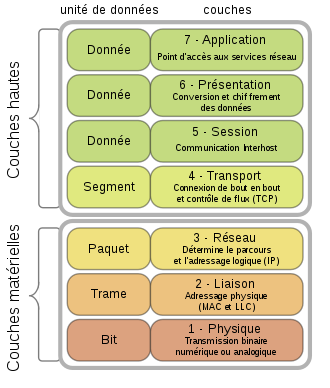
\includegraphics[height=.3\textheight]{images/osi/reseau_OSI}
  \caption{Les couches du modèle OSI}
  \label{fig:res_osi}
\end{figure}

\subsection{Les couches matérielles}
\label{sec:couches}
Ce sont celles qui assurent la liaison matérielle entre les organes. C'est cette couche qui s'assure qu'un paquet envoyé par un expéditeur $E$ arrive bien jusqu'au destinataire $D$.
\paragraph{Couche 1 : Couche physique}
\begin{description}
  \item [Nom : ] Couche Physique
  \item [Rôle : ] Offrir un support de transmission pour la communication
  \item [Rôle secondaire : ] Néant
  \item [Exemple de matériel associé : ] Concentrateur (cf \ref{sec:concentrateur})
\end{description}

\paragraph{Couche 2 : Couche liaison}
\begin{description}
  \item [Nom : ] Liaison de donnée
  \item [Rôle : ] Connecter les machines entre elles sur un réseau local.
  \item [Rôle secondaire : ] Détecter les erreurs de transmission.
  \item [Exemple de matériel associé : ] Commutateur (cf \ref{sec:commutateur})
\end{description}


\paragraph{Couche 3 : Couche réseau}
\begin{description}
  \item [Nom : ] Réseau
  \item [Rôle : ] Interconnecter les réseaux entre eux.
  \item [Rôle secondaire : ] Fragmenter les paquets.
  \item [Exemple de matériel associé : ] Routeur (cf \ref{sec:routeur})
\end{description}

\subsection{Les couches hautes}
Les couches hautes sont la plupart du temps logicielles. Elle permettent de faire le lien entre le paquet et l'utilisation que l'on fait de ce paquet. Dans les cours de ce module, nous nous intéresserons principalement aux couches matérielles ainsi qu'aux couches 4 et 7 et laisserons de côté les couches 5 et 6.

\paragraph{Couche 4 : Couche transport}
\begin{description}
  \item [Nom : ] Couche Transport
  \item [Rôle : ] gérer les connexions applicatives.
  \item [Rôle secondaire : ] garantir la connexion.
\end{description}


\paragraph{Couche 7 : Couche Application}
\begin{description}
  \item [Nom : ] Application
  \item [Rôle : ] ?
  \item [Rôle secondaire : ] ?
\end{description}
Cette couche représente l'application utilisant les paquets qui transitent sur le réseau. Elle n'a donc pas de rôle précis associé puisque cela dépendra de l'application.

\subsection{Le modèle OSI : une norme}
Le modèle OSI est une  norme, cela signifie qu'il définit des règles que les concepteurs de réseaux doivent suivre. Si chaque intervenant respecte la norme, alors le modèle OSI garantit le bon fonctionnement du réseau. Les matériels sont donc fabriqués selon cette norme afin d'assurer la compatibilité entre ces composants.

Ainsi, chaque couche doit remplir son rôle et uniquement son rôle. Deux règles générales entre les couches s'ajoutent :
\begin{itemize}
  \item Chaque couche est indépendante
  \begin{itemize}
    \item Les informations utilisées par une couche ne pourront pas être utilisées par une autre couche.
Par exemple, pour ceux qui connaissent déjà un peu le réseau, l'adresse IP qui est une adresse de couche 3 ne pourra pas être utilisée par une autre couche, sous peine de ne pas respecter le modèle OSI.
  \item Cela permet notamment de garantir l'évolution des communications dans le temps.
  \end{itemize}
  \item Chaque couche ne peut communiquer qu'avec une couche adjacente
  \begin{itemize}
    \item Pour envoyer une information, une appliction (couche 7) transmettra son paquet à la couche 6 qui le traitera et le passera à la couche 5 et ainsi de suite jusqu'à la couche 1.
    \item A la réception, le paquet remonte les couches jusqu'à la couche 7 de la l'application destinaire.
  \end{itemize}
\end{itemize}
